% !Mode:: "TeX:UTF-8:Main"

% slow play!
% music:
% 0:00 - 0:30
% https://www.youtube.com/watch?v=WYeDsa4Tw0c&t=5s
 
\documentclass[aspectratio=169]{beamer}

\usepackage{tikz}
\usetikzlibrary{ducks}
\usetikzlibrary {decorations.markings}

\setbeamertemplate{navigation symbols}{}
\setbeamertemplate{background canvas}{\makebox[\paperwidth]
{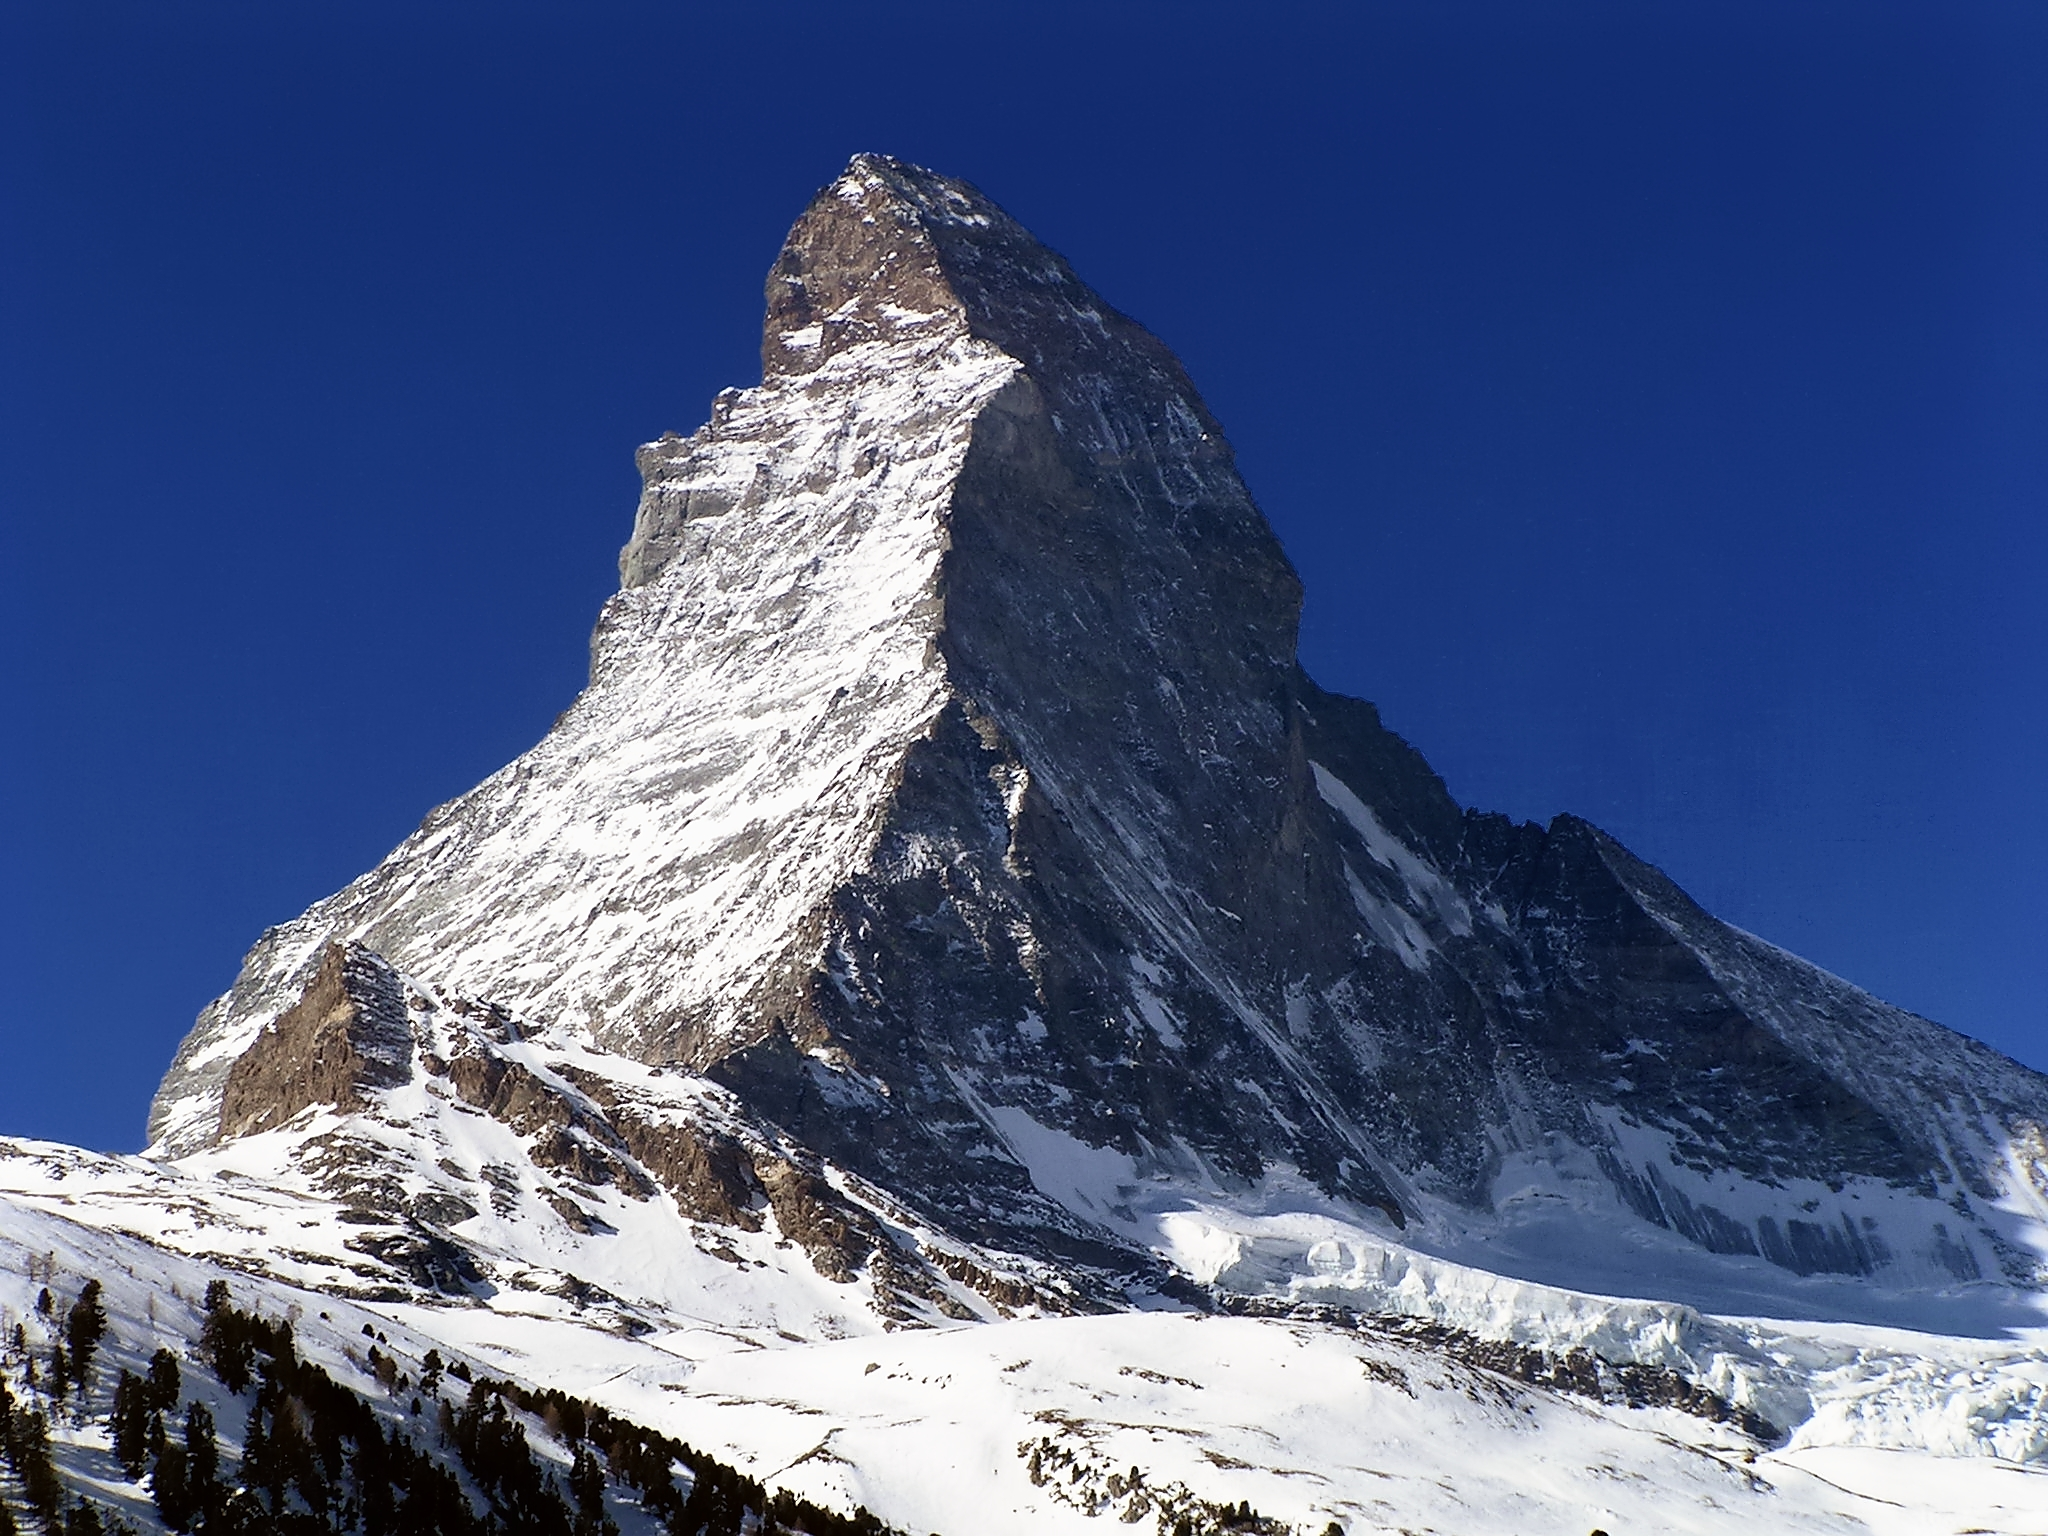
\includegraphics[width=0.9\paperwidth,trim=0cm 0cm 0cm 5cm]
  {Matterhorn-EastAndNorthside-viewedFromZermatt_landscapeformat-2}}}

%\newcommand\calcpos[1]{\fpeval{(trunc(\value{page}/4))/200*22+#1}cm}
\newcommand\calcpos[1]{\fpeval{(\value{page})/800*22+#1}cm}
\begin{document}
	
%\end{document}
\begin{frame}
  \begin{tikzpicture}[%
  remember picture,
  decoration={
  markings,
  %mark= at position 0cm with {\node{
\includegraphics[scale=0.2]{duck}};},
    mark= at position \calcpos{0}
    with {\node{
\includegraphics[scale=0.3]{duck}};}, 
  mark= at position \calcpos{0.6}
    with {\node{
\includegraphics[scale=0.23,page=2]{duck}};}, 
    mark= at position \calcpos{1.2}
    with {\node{
\includegraphics[scale=0.23]{duck}};},
     mark= at position \calcpos{1.8}
    with {\node{
\includegraphics[scale=0.3,page=2]{duck}};},    
  %mark= at position 22cm with {\node{
\includegraphics[scale=0.2]{duck}};}
  }
  ]
   \path[use as bounding box](0,0)rectangle(\textwidth,\textheight-15pt);  
   \path[%draw=red,thick,
   postaction=decorate] 
   (15,0.2) 
   --  (10.1,0.75)
   -- (9,1)
   -- (8,1)
   -- 
   (7,0.6)
   -- (6,1)
   -- (5,1.7)
   -- (4,2)
   -- (3,2.6)
   -- (2.1,3)
   -- (4,3.2)
   -- (5,3.8)
   -- (4,4.2)
   -- (6,5)
   -- (5,6)
   -- (6.4,6.8);
    
    % credit for background image
    \node[font=\tiny,align=center] at 
     ([yshift=0.35cm]current page.south) {Image source: \url{https://commons.wikimedia.org/wiki/File:Matterhorn-EastAndNorthside-viewedFromZermatt_landscapeformat-2.jpg}};  
    
  \end{tikzpicture}
  \pause[769]
\end{frame}	
	
\end{document}
